\section{HAT deska plošných spojů}
Pro ovládání výše popsaného hardwaru je~zapotřebí několik specifických obvodů.
Kvůli jejich specifičnosti tyto obvody nejsou volně dostupné k~zakoupení na~předem vytvořených destičkách. Proto bylo zapotřebí je~z~jednotlivých součástek vyrobit na~míru.

Obvody byly navrženy v~programu KiCad, celé schéma desky je~k~nalezení v~příloze~1 na~konci tohoto dokumentu. Další výrobní dokumenty z~programu KiCad jsou k~nalezení v~souborové příloze ve~složce \uv{pcb}. Následně pro~ně v~tomtéž programu byla nadesignována deska plošných spojů. Mezi obvody patří:
\begin{itemize}
  \item Zdroj $-15$~V~pro galvanometry.
  \item Generátor signálu pro~řídící desku galvanometrů.
  \item Voltmetr baterií.
\end{itemize}

Kromě nich byly na~desku přidány konektory k~jednotlivým barevným vstupům laseru, LCD~displeji a~k~rotačnímu enkodéru, které jsou přímo napojeny na~40 pinový GPIO konektor Raspberry Pi.
Deska byla designována jako tzv. HAT, to~znamená, že sama na~tomto konektoru drží a~nezabírá o~moc~víc místa, než samotné Raspberry Pi. Deska připevněná na RPi je vidět na obrázku~\ref{fig:pcb-mounted}

\begin{figure}[htb]
  \centering
  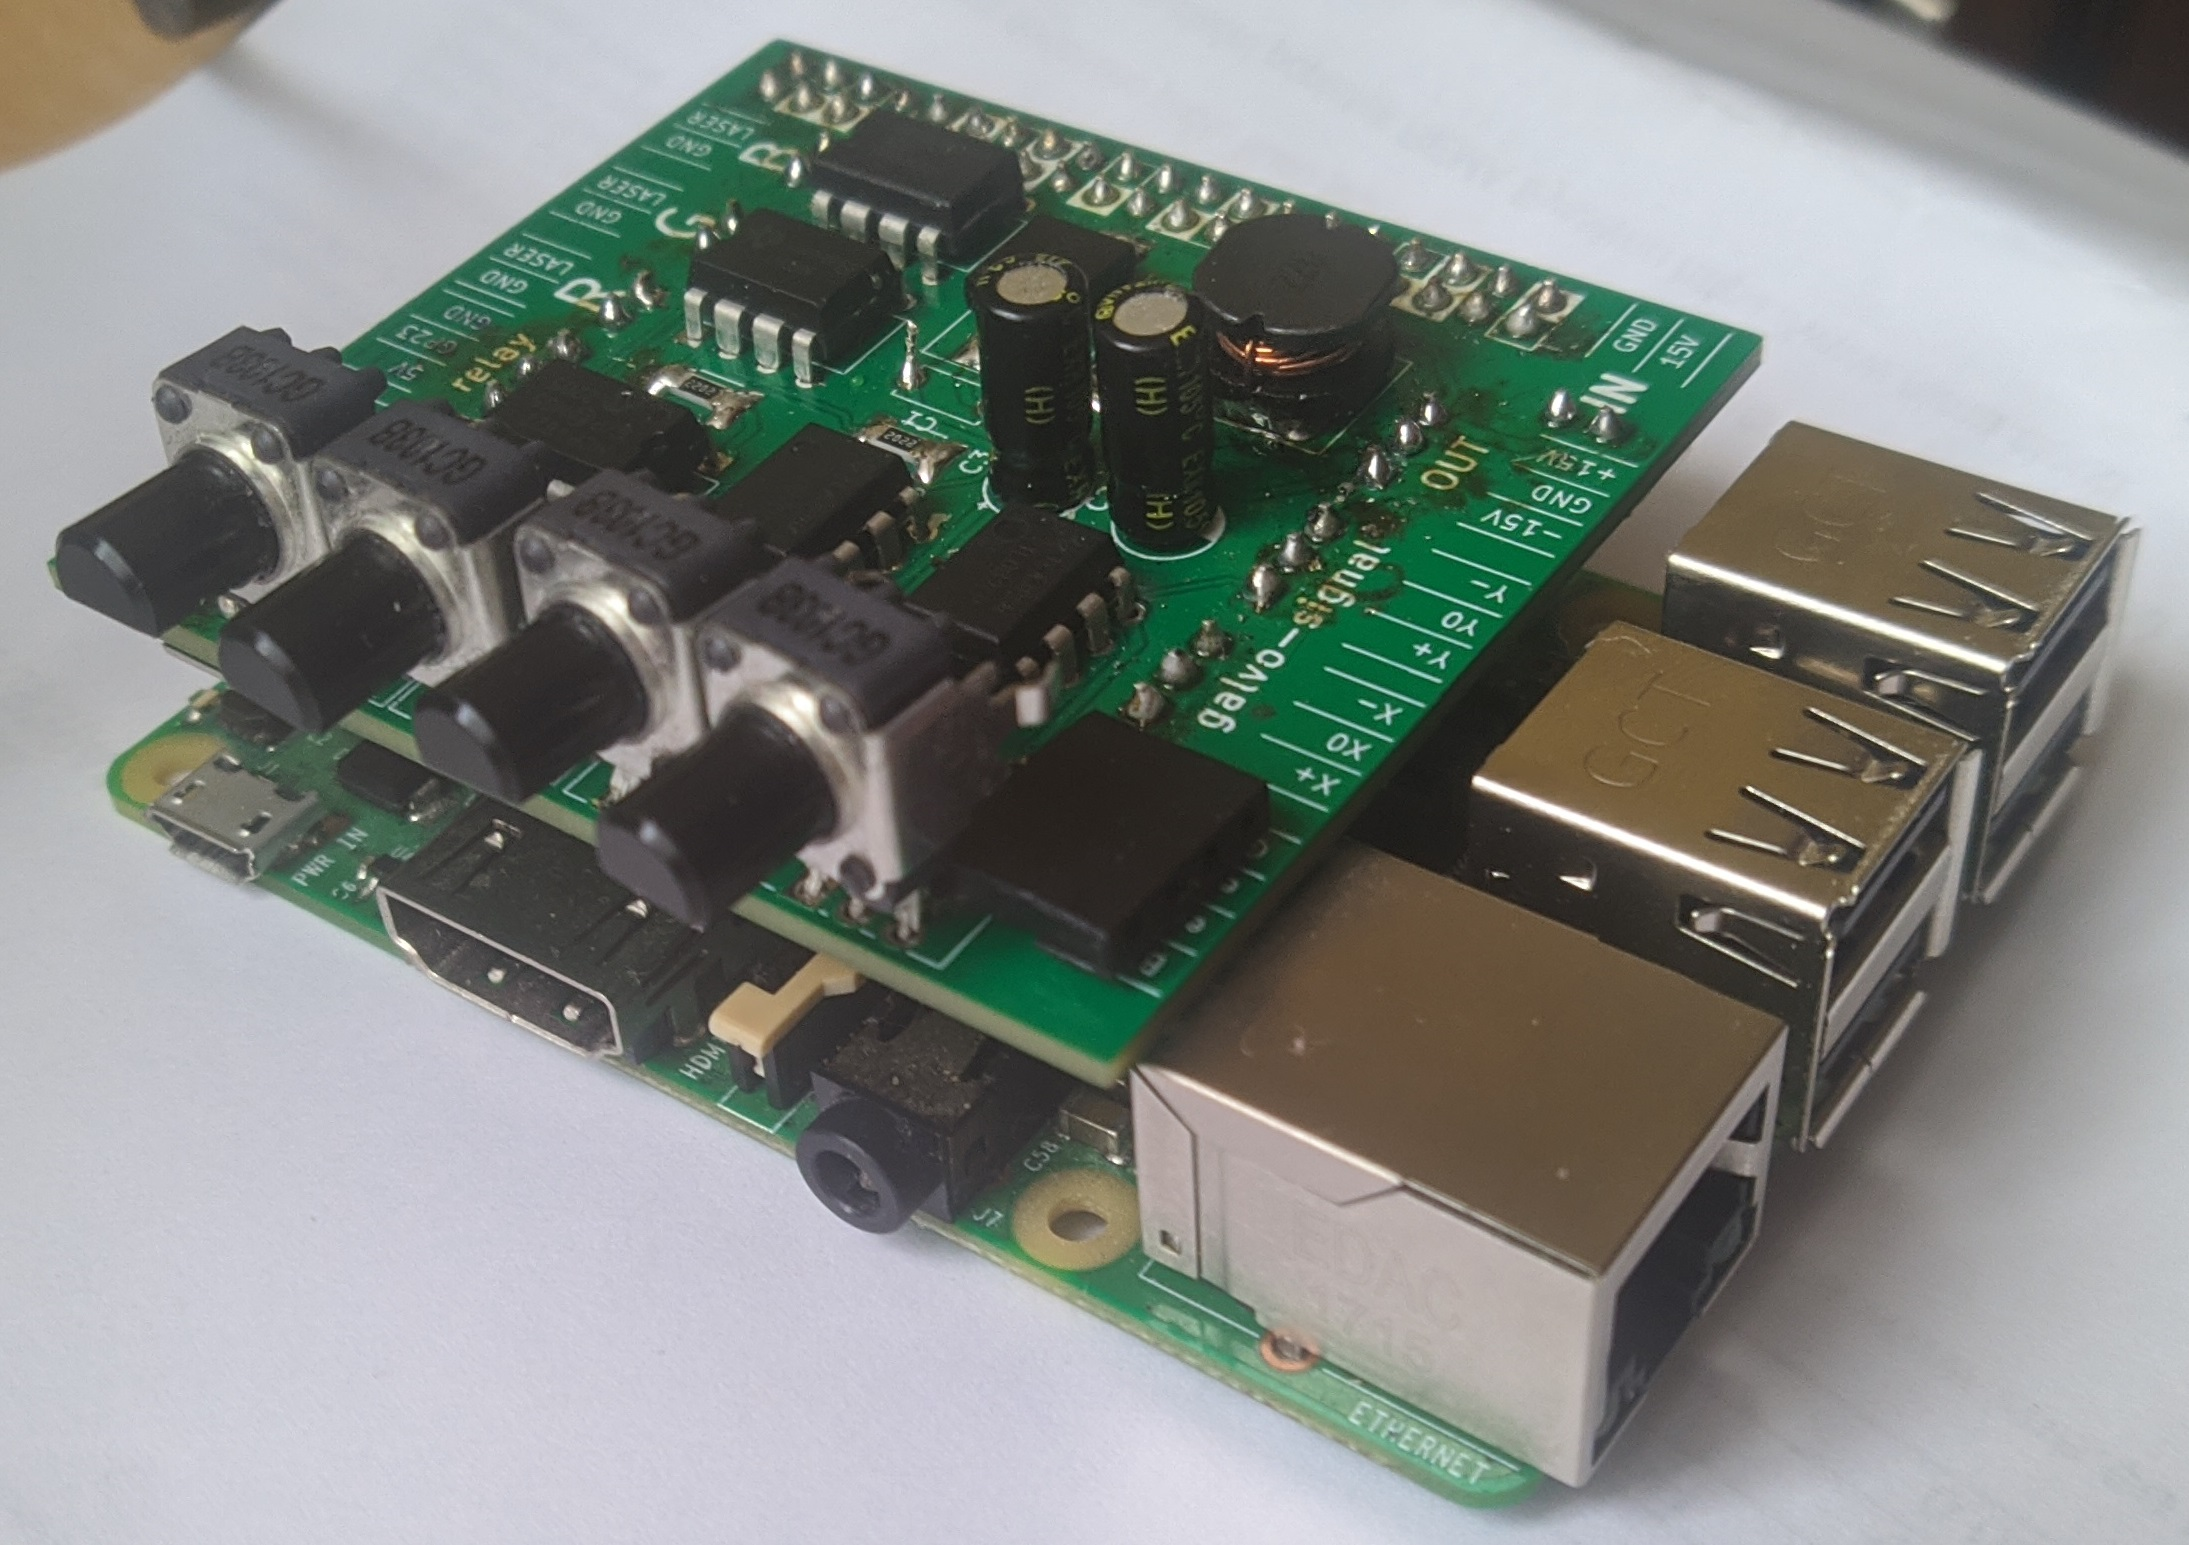
\includegraphics[width=0.6\textwidth]{img/pcb-mounted.jpg}
  \caption{\label{fig:pcb-mounted} HAT DPS připevněná na Raspberry Pi }
\end{figure}

\subsection{Zdroj $-15$~V}\label{sec:negative-ps}
Napětí $-15$~V~je~získáváno obvodem napěťového invertoru založeném na~obvodu ze~zdroje~\cite{ampalyzer}. Jeho zapojení je~na~obrázku~\ref{fig:negative-ps}, potřebuje zdroj napětí 15~V.

V aktuálním stavu tento zdroj nefunguje, to~bude brzo napraveno. Zatím je zařízení napájeno vnějším zdrojem, který dodává $+15$~V i~$-15$~V.

\begin{figure}[htb]
  \centering
  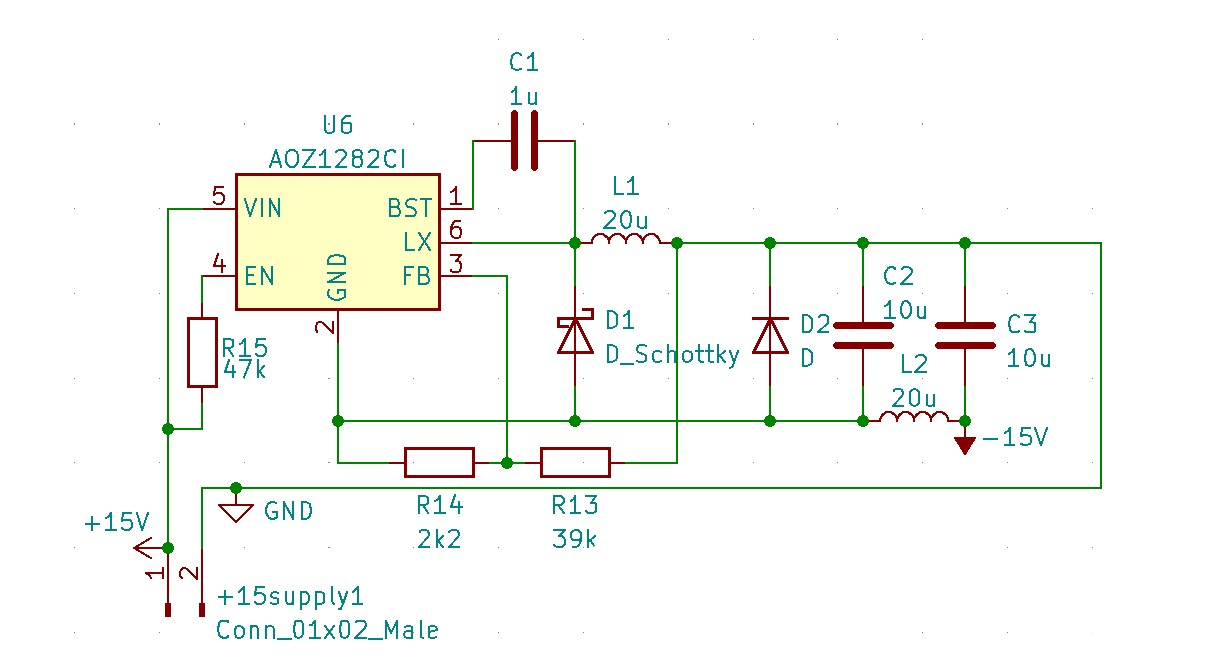
\includegraphics[width=0.9\textwidth]{img/negative-ps.jpg}
  \caption{\label{fig:negative-ps} Zapojení invertujícího obvodu}
\end{figure}

Centrem obvodu je~integrovaný obvod AOZ1282 od~výrobce Alpha \& Omega Semiconductor označený U6. Tento integrovaný obvod obsahuje spínací transistor (ve~zjednodušeném schématu prvek SW), PWM~regulační obvod pracující na~frekvenci 450 kHz~s napěťovou referencí 0,8 V, který reguluje čas připojení induktoru L1.
K němu je~připojen bootstrapový kondenzátor C1, ten~zajišťuje plovoucí buzení pro~integrovaný spínač.
Dále je~k~němu připojený výkonový induktor L1, jehož hodnota byla zvolena dle~rovnic uvedených ve~zdroji~\cite{basic-calc-boost}, respektive podle dále uvedené rovnice~\ref{equ:inductor-calc}.~\cite{ampalyzer}

\begin{equ}[H]
  \centering
  \begin{math}
     L~= \frac{-U_{OUT}\times U_{IN}}{0,4 \times 2 \times I_{OUT} \times f_{s} \times \left ( U_{IN} - U_{OUT} \right )} = \frac{- \left (-15 V~\right )\times 15 V}{0,4 \times 2 \times 1 A~\times 450 kHz~\times \left ( 15 V~- \left (-15 V~\right ) \right )} \approx 21 \mu~H
  \end{math}
  \caption{\label{equ:inductor-calc} Výpočet ideální indukčnosti cívky pro~invertující obvod}
\end{equ}

\It{
   L~--- Indukčnost spínaného induktoru \\
  U$_{IN}$ --- Vstupní napětí do~invertujícího obvodu \\
  U$_{OUT}$ --- Výstupní napětí z~invertujícího obvodu \\
  I$_{OUT}$ --- Výstupní proud z~invertujícího obvodu \\
  f$_{s}$ --- Frekvence spínacího regulátoru \\
}

Na FB~pin~integrovaného obvodu je~připojen napěťový dělič tvořený odpory R13 a~R14, který integrovanému obvodu dodává zpětnou vazbu o~výstupním napětí.
Hodnoty R13 a~R14 jsou voleny tak, aby~při 15 V, tedy požadovaném výstupním napětí, bylo na~výstupu děliče napětí 0,8 V, tedy referenční napětí integrovaného spínaného regulátoru.
Schottkyho dioda SS56, označená D1, slouží k~zadržení změny polarity induktoru. Usměrňovací dioda D2 je~v~propustném stavu při prvotním spuštění měniče, kdy~je~přes ní napájen U1 po~dobu náběhu výstupního záporného napětí.
Posledním prvkem je~výstupní vyhlazovací filtr tvořený kondenzátory C3 a~C4 společně s~induktorem L2.
Jeho úkol je~minimalizovat výstupní napěťového zvlnění zdroje.~\cite{ampalyzer}

\subsection{Generátor analogového signálu}\label{sec:ilda-signal-gen}
Jak je~popsáno v~sekci~\ref{sec:my-galvos}, řídící deska galvanometrů přijmá dva~bipolární diferenciální analogové signály v~rozpětí $-5$~V~až $+5$~V.

Obvod, který se~stará o~vytváření tohoto signálu, je~založený na~obvodu ze~zdroje~\cite{lasershow-with-real-galvos}.
Vytváření tohoto signálu je~rozděleno do~dvou částí. Nejdříve D/A~převodník připojený k~RPi~vytvoří signál v~rozpětí 0 až 5~V~a~následně je~tento signál pomocí invertujících operačních zesilovačů převeden na~požadované rozpětí a~invertován.
Jednotlivé části tohoto obvodu jsou blíže popsány v~následujících kapitolách.

\subsubsection{D/A převodník}
K generování signálu v~rozpětí 0--5~V~byl využit dvoukanálový D/A převodník\footnote{D/A převodník je~obvod, který na~základě instrukcí přijatých digitálně generuje analogové napětí.} MCP4822.
Tento čip podporuje komunikaci přes rozhraní SPI, pracuje s~napájecím napětím 5~V~a~s~12bitovým rozlišením (je schopen vygenerovat 4~096 různých napětí) na~dvou kanálech~\cite{mcp4822-dsh}.
RPi komunikuje s~čipem pomocí rozhraní SPI~popsaném v~kapitole~\ref{sec:spi}.

\subsubsection{Operační zesilovače}
K modifikaci signálu z~DAC~na~bipolární diferenciální analogový signál slouží pro~každý kanál jeden čip TL082~\cite{tl082-dsh}, který obsahuje dva~operační zesilovače. Ty~jsou zapojeny dle~schématu na~obrázku~\ref{fig:ilda_amps-scheme}.

Signál první operační zesilovač zesílí/zeslabí a~vertikálně posune dle~nastavení potenciometrů Ygain (zesílení) a~Yoffset (posun) a~zároveň invertuje. Tento invertovaný signál následně druhý operační zesilovač opět invertuje. Tím získavá základní signál pro~řídící desku galvanometrů.

\begin{figure}[htb]
  \centering
  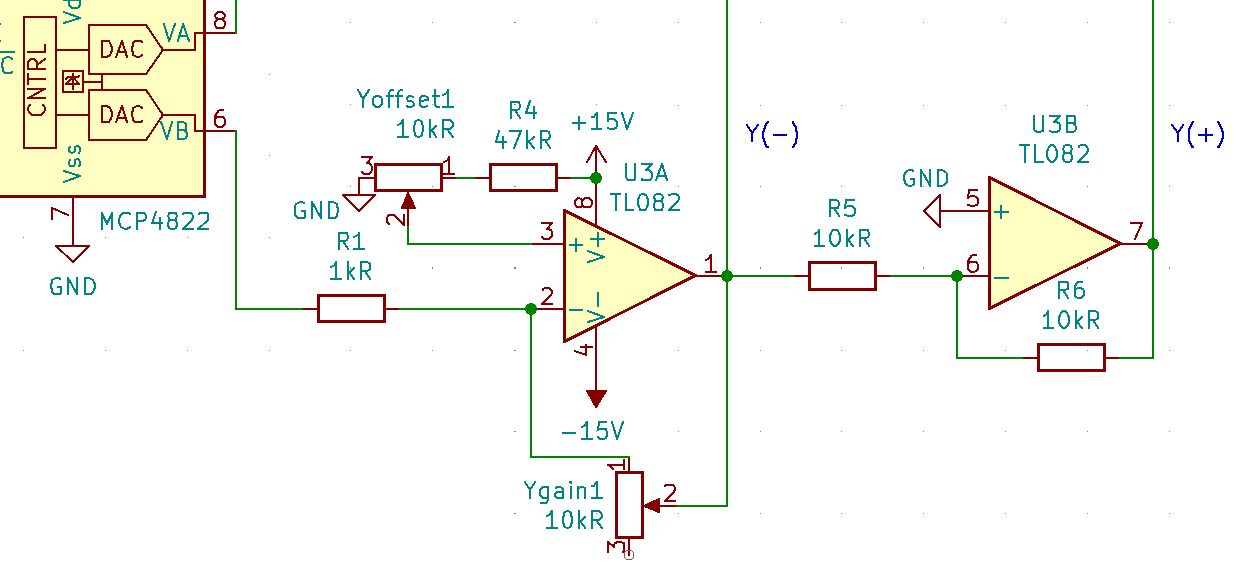
\includegraphics[width=1\textwidth]{img/ilda_amps.png}
  \caption{\label{fig:ilda_amps-scheme} Zapojení čipu TL082 pro~jeden kanál řídící desky galvanometrů}
\end{figure}

\subsection{Voltmetr baterií}
Obvod voltmetru baterií je~vidět na~obrázku~\ref{fig:bat_probe}.

\begin{figure}[htb]
  \centering
  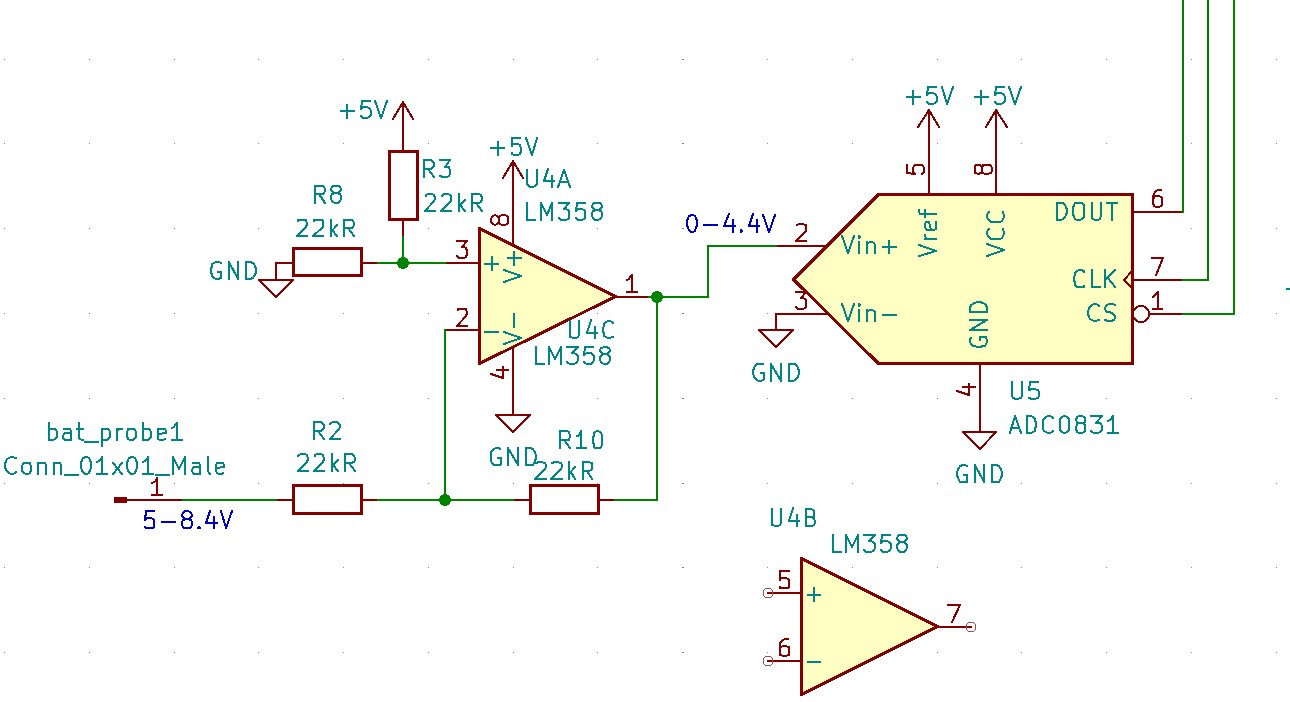
\includegraphics[width=0.6\textwidth]{img/bat_probe.jpg}
  \caption{\label{fig:bat_probe} Schéma obvodu voltmetru baterie}
\end{figure}

Jako voltmetr baterií slouží A/D převodník ADC0831 od~firmy Texas Instruments Incorporated~\cite{adc0831-dsh}. Ten~je~označen U5 a~je~zapojen společně s~operačním zesilovačem LM358 od~stejného výrobce, který je~označen U4.
Operační zesilovač je~zapojen jako rozdílový zesilovač podle zdroje~\cite{odcitacka} tak, aby~od~napětí baterií, které se~může pohybovat v~rozsahu 6~V~až 8,4~V, odečítal 5~V.
Díky tomu se~napětí, která měří A/D převodník pohybují mezi hodnotami 1~V~a 3,4~V. S~jeho osmibitovým rozlišením a~referenčním napětím 5~V~v tomto rozpětí může naměřit 122 různých napětí.

A/D převodník tyto data posílá do~Raspberry Pi~pomocí rozhraní SPI~a to~s~nimi dále pracuje.
